\chapter{通信架构}
\label{cha:Communication}

\section{串行通信}

在本项目中异步串行通信主要用于本地系统内的通信,远程通信有相应模块转换。

发送端在发送串行数据的同时,提供一个时钟信号,并按照一定的约定(例如在时钟信号的上升沿的时候,将数据发送出去)发送数据,接收端根据发送端提供的时钟信号,以及约定,接收数据。这就是同步串行通信(Synchronous serial communication),I2C、SPI等有时钟信号的协议,都属于这种通信方式。

% 发送端在数据发送之前和之后,通过特定形式的信号(例如START信号和STOP信号),告诉接收端,可以开始(或者停止)接收数据了。与此同时,收发两方会约定一个数据发送的速度(波特率),发送端在发送START信号之后,就按照固定的节奏发送串行数据,与此同时,接收端在收到START信号之后,也按照固定的节奏接收串行数据。这就是异步串行通信(Asynchronous serial communication),串口通信,就是这种通信方式。

UART(Universal Asynchronous Receiver/Transmitter) 即是规定编码格式、bit rate,产生通信所需的bit流的标准。

COM (通信端口)是最早的但仍极为常用的PC兼容机串口,不仅指物理端口,也指虚拟端口,如蓝牙或USB创建的串口。

\subsection{UART}

\begin{figure}[htbp]
    \centering
    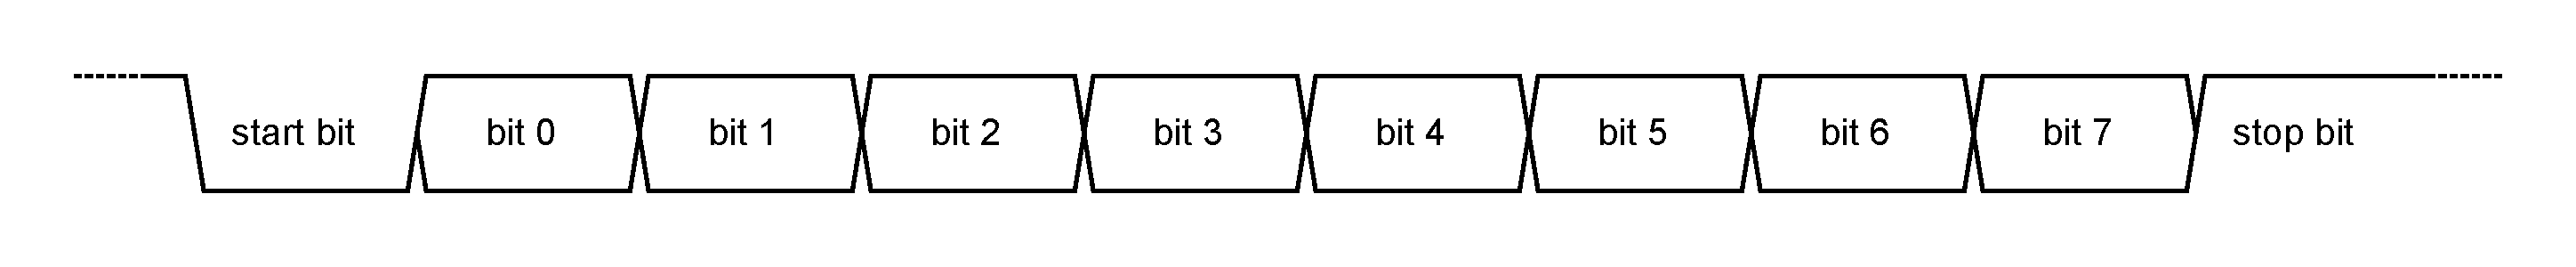
\includegraphics[width=\columnwidth]{UART_timing_diagram.pdf}
    \caption{UART数据帧}
    \label{fig:UART-Data-framing}
\end{figure}

% 通用异步收发传输器(Universal Asynchronous Receiver/Transmitter,通常称为UART),如图~\ref{fig:UART},是一种异步收发传输器,是电脑硬件的一部分,将数据透过串列通讯和平行通讯间作传输转换。UART通常用在与其他通讯接口(如EIA RS-232)的连接上。\footnote{\url{https://en.wikipedia.org/wiki/Universal_asynchronous_receiver-transmitter}}

% 具体实物表现为独立的模组化芯片,或是微处理器中的内部周边装置(peripheral)。一般和RS-232C规格的,类似Maxim的MAX232之类的标准信号幅度变换芯片进行搭配,作为连接外部设备的接口。在UART上追加同步方式的序列信号变换电路的产品,被称为USART(Universal Synchronous Asynchronous Receiver Transmitter)。

我们的Arduino编程器的通信协议就是UART\footnote{\url{https://en.wikipedia.org/wiki/Universal_asynchronous_receiver-transmitter}},如图~\ref{fig:UART}。一般MCU芯片之间的通信协议都是UART。

\begin{figure}[htbp]
    \centering
    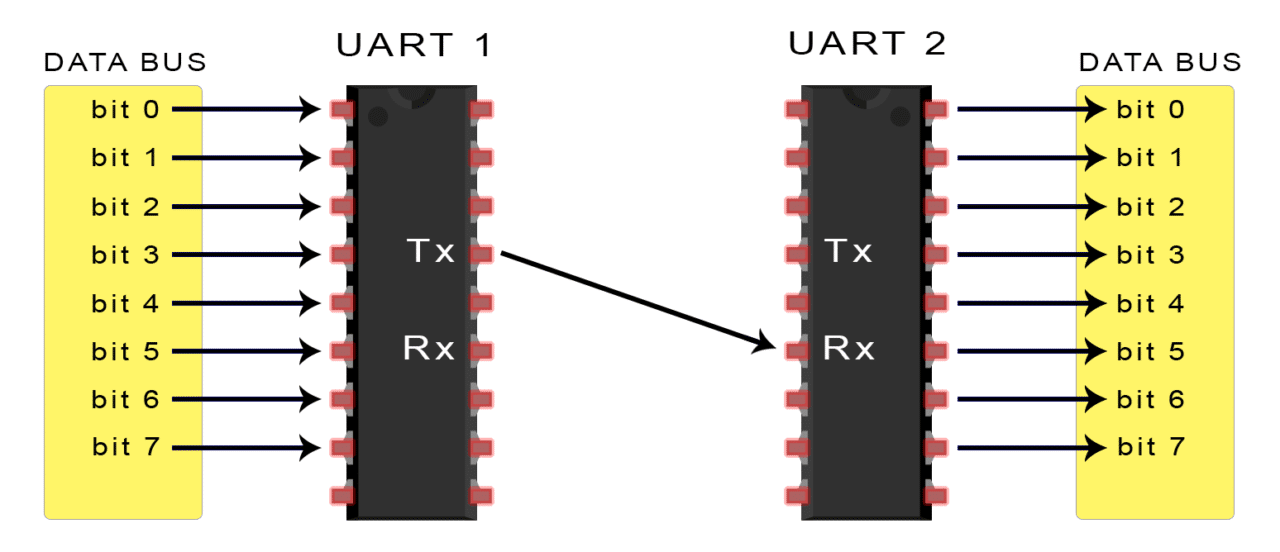
\includegraphics[width=\columnwidth]{Introduction-to-UART-Data-Transmission-Diagram.png}
    \caption{UART}
    \label{fig:UART}
\end{figure}

\subsection{USB}

% 通用串行总线(英语:Universal Serial Bus,缩写:USB)是连接计算机系统与外部设备的一种串口总线标准,也是一种输入输出接口的技术规范,被广泛地应用于个人电脑和移动设备等信息通讯产品,并扩展至摄影器材、数字电视(机顶盒)、游戏机等其它相关领域。

\begin{figure}[htbp]
    \centering
    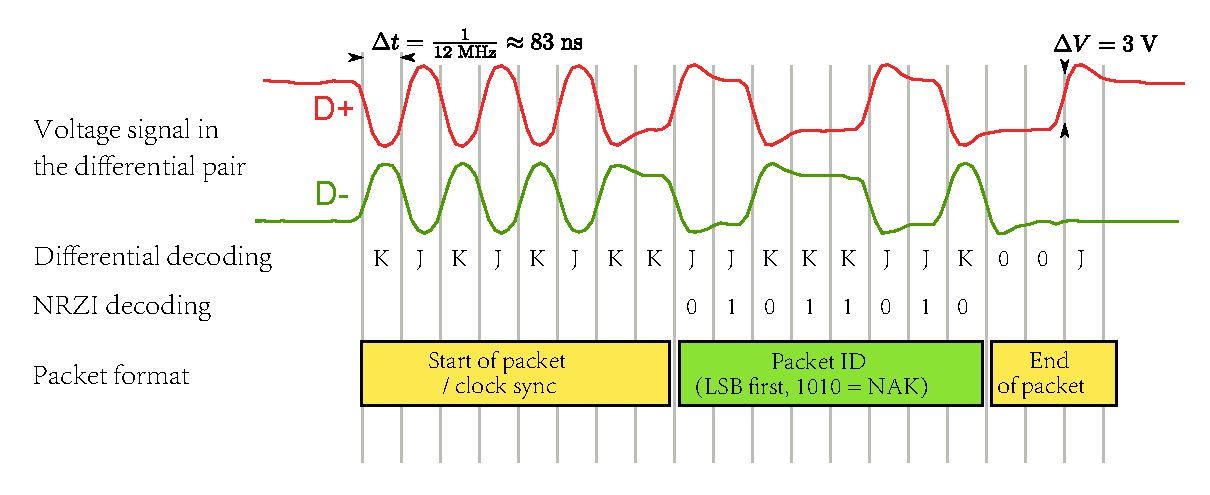
\includegraphics[width=\columnwidth]{USB_signal_example.pdf}
    \caption{Transmission example on a USB 1.1 full-speed device}
    \label{fig:USB-Transmission}
\end{figure}

USB传输协议见\url{https://en.wikipedia.org/wiki/USB_(Communications)#Protocol_layer}。其半双工传输模式如图~\ref{fig:USB-Transmission}。

% BOT传输协议:BOT (Bulk-Only Transport),诞生于1999年,专为USB 1.1所设计,至今最快的USB 3.1都可向下兼容这个基本的BOT传输协议。在传输数据作业开始时,外接USB 3.0设备与电脑主板(USB 3.0扩展卡)之间,在同一时间单位内,每次只传输单一指令,所以速度较UASP慢,属于“半双工传输模式”,如图~\ref{fig:USB-Transmission}。

% 在数据传输量大的情况下可以使用UASP传输协议(USB Attached SCSI Protocol),需USB 3.0以上方能使用。与USB 3.0一同诞生于2008年,USB应用者论坛(USB-IF)为改良BOT传输协议过慢的缺点,将SCSI架构改进并推出UASP,包括多命令平行处理能力、任务管理与控制等机制,也支持NCQ(原生指令排序),速度比BOT传输模式快上许多,属于“全双工传输模式”。UASP的设备端桥接芯片有:LucidPort USB 300、祥硕科技ASMedia ASM1053/ASM1042、智微JMS 569、德州仪器TUSB9261等等。

% \subsection{RS-232}

% RS-232, Recommended Standard 232 \footnote{RS-232, when compared to later interfaces such as RS-422, RS-485 and Ethernet, has lower transmission speed, short maximum cable length, large voltage swing, large standard connectors, no multipoint capability and limited multidrop capability. In modern personal computers, USB has displaced RS-232 from most of its peripheral interface roles.} 是一种串行通信协议。见\url{https://en.wikipedia.org/wiki/RS-232}

% RS232或者RS485,它更多的是规定电气特性和各个引脚的功能定义,如 用-3V - -15V之间的任意电平表示逻辑“1” ;用+3V - +15V电平表示逻辑“0”,这里采用的是负逻辑。



\section{ROS节点通信测试平台选型}

我们选用Nvidia Jetson NANO(如图~\ref{fig:Jetson-Nano})作为主要的开发平台,NVIDIA Jetson Nano开发人员工具包是一台功能强大的小型计算机,可并行运行多个神经网络,以用于图像分类,对象检测,分段和语音处理等应用,该平台的功耗仅为5瓦。

\begin{figure}[htbp] % use float package if you want it here
    \centering
    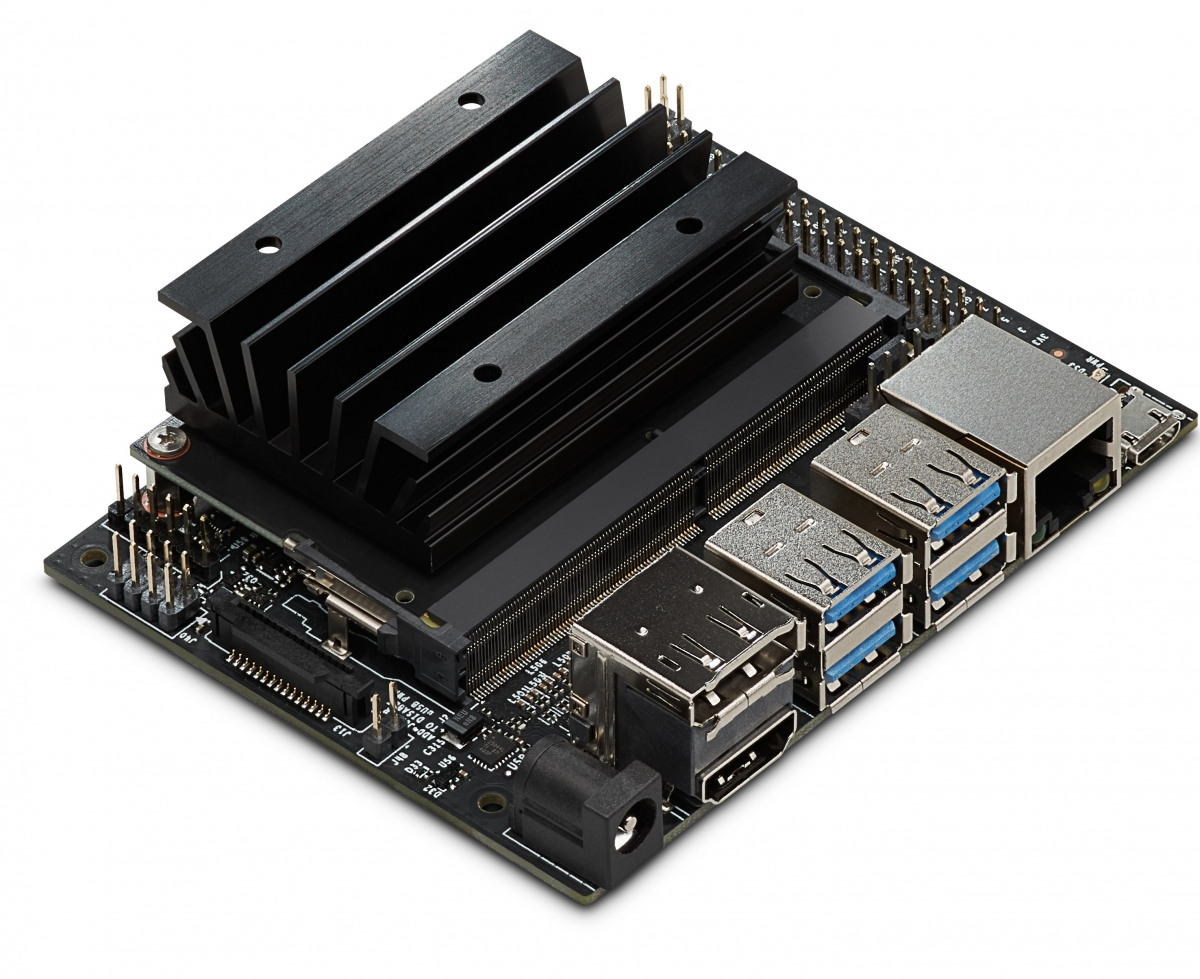
\includegraphics[height=6cm]{Jetson-Nano.jpg}
    \caption{Nvidia Jetson NANO}
    \label{fig:Jetson-Nano}
\end{figure}

初步的硬件平台,采用无线局域网通信,图~\ref{fig:wifi}为将AC8265和片状5GHz天线装到Jetson Nano Developer Kit上。

\begin{figure}[htbp]
    \begin{minipage}{0.48\textwidth}
      \centering
      \includegraphics[height=5cm]{DA4A3052.JPG}
      \caption{为Nano添加无线网功能}
      \label{fig:wifi}
    \end{minipage}\hfill
    \begin{minipage}{0.48\textwidth}
      \centering
      \includegraphics[height=5cm]{DA4A3066.JPG}
      \caption{两机组通信测试平台}
      \label{fig:two-setup}
    \end{minipage}
\end{figure}

